\begin{frame}{Kiến trúc RAG - Giai đoạn Lập chỉ mục (Indexing)}
\begin{figure}[H]
\centering
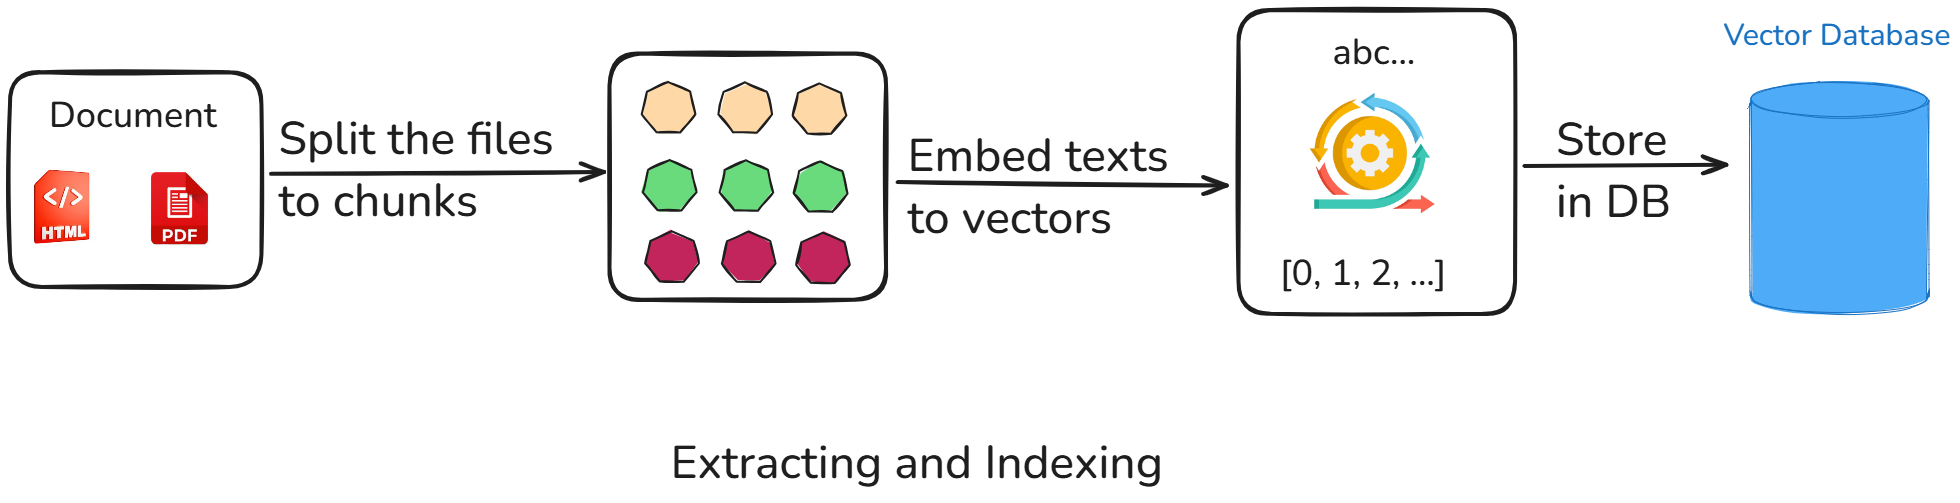
\includegraphics[height=0.55\textheight,width=0.9\textwidth,keepaspectratio]{pictures/rag-1.excalidraw.png}
\caption{Sơ đồ RAG cơ bản (Extracting and Indexing)}
\end{figure}

\note{
Để giải quyết nhược điểm của LLM, kiến trúc RAG được áp dụng. Giai đoạn đầu tiên là Lập chỉ mục (Indexing).
Toàn bộ tài liệu tri thức (văn bản luật, tài liệu nội bộ) được chia nhỏ thành các đoạn (chunks). Sau đó, hệ thống sử dụng mô hình nhúng (embedding models) để chuyển đổi các đoạn văn bản này thành các biểu diễn vector và lưu trữ vào Vector Database để tối ưu hóa việc tìm kiếm.
}
\end{frame}
